\documentclass{standalone}

\usepackage[OT1]{fontenc}
\renewcommand*\familydefault{\sfdefault}
\usepackage{helvet,sfmath}
\usepackage{siunitx}

\usepackage{tikz}
\usetikzlibrary{arrows,calc,patterns}
% \usetikzlibrary{intersections, calc, arrows.meta}
\usepackage{tikz,tkz-euclide}

\begin{document}
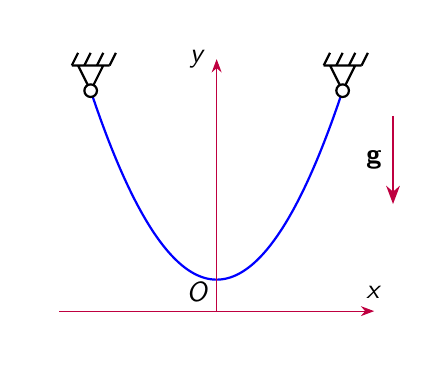
\begin{tikzpicture}[scale=0.8, >=Stealth]

    %% Background
    \draw[draw=none] (-3,-1) rectangle (3,4);

    % Catenary
    \draw[thick, blue, domain=-2:2, samples = 100, smooth, variable=\t] 
    plot ({\t}, {0.75*\t*\t});

    \draw[thick]
    (-2,3) to (-1.8,3.4)
    (-2,3) to (-2.2,3.4)
    (-1.7,3.4) to (-2.3,3.4)
    (2,3) to (1.8,3.4)
    (2,3) to (2.2,3.4)
    (1.7,3.4) to (2.3,3.4)
    ;

    \foreach \x in {-2.3,-2.1,-1.9,-1.7}
    {
    \draw[thick] (\x,3.4) to (\x+0.1,3.6);
    }
    \foreach \x in {2.3,2.1,1.9,1.7}
    {
    \draw[thick] (\x,3.4) to (\x+0.1,3.6);
    }

    \draw[thick, fill=white]
    (-2,3) circle (0.1)
    (2,3) circle (0.1)
    ;

    %Coordinate
    \draw[purple, -Stealth] (-2.5,-0.5) to (2.5,-0.5);
    \draw[purple, -Stealth] (0,-0.5) to (0,3.5);

    \draw
    (-0.3,3.5) node{\(y\)}
    (2.5,-0.2) node{\(x\)}
    (-0.3,-0.2) node{\(O\)}
    ;

    %Gravity
    \draw[thick, purple, -Stealth] (2.8,2.6) to (2.8,1.2);
    \draw
    (2.5,1.9) node{\(\mathbf{g}\)}
    ;
    
\end{tikzpicture}
\end{document}